%% Intended to be included into a larger document
\chapter{Related Work}
\label{cha:related-work}

This chapter examines related research in this area. The related work on Serious game and and the recent development of gamification is discussed in Section 2.1 and Section 2.2. Section 2.3 looks at the applications of ``serious game'' in the sustainability context. Finally, Section 2.4 and 2.5 examines the serious game framework and its assessment.

%% Add more to introduce topics in this chapter?
\section {Serious Game}
A Serious game is a complete game designed for a primary purpose other than pure entertainment \cite {WikipediaSeriousGame}. It includes categories such as educational games and advergames (advertising), political games, and training game (also known as game-learning). Zyda (2005) defines serious game is "a mental contest, played with a computer in accordance with specific rules that uses entertainment to further government or corporate training, education, health,etc".

One example is Fold.it, which made the headline \cite {khatib2011crystal} by using game play to help solve problems that computers cannot solve very well, in this case, online gamers were able to do what biochemists have been trying to do for a decade: decipher the structure of a protein that is key to the way HIV multiplies.

\begin{figure}[htbp]
	\centering
		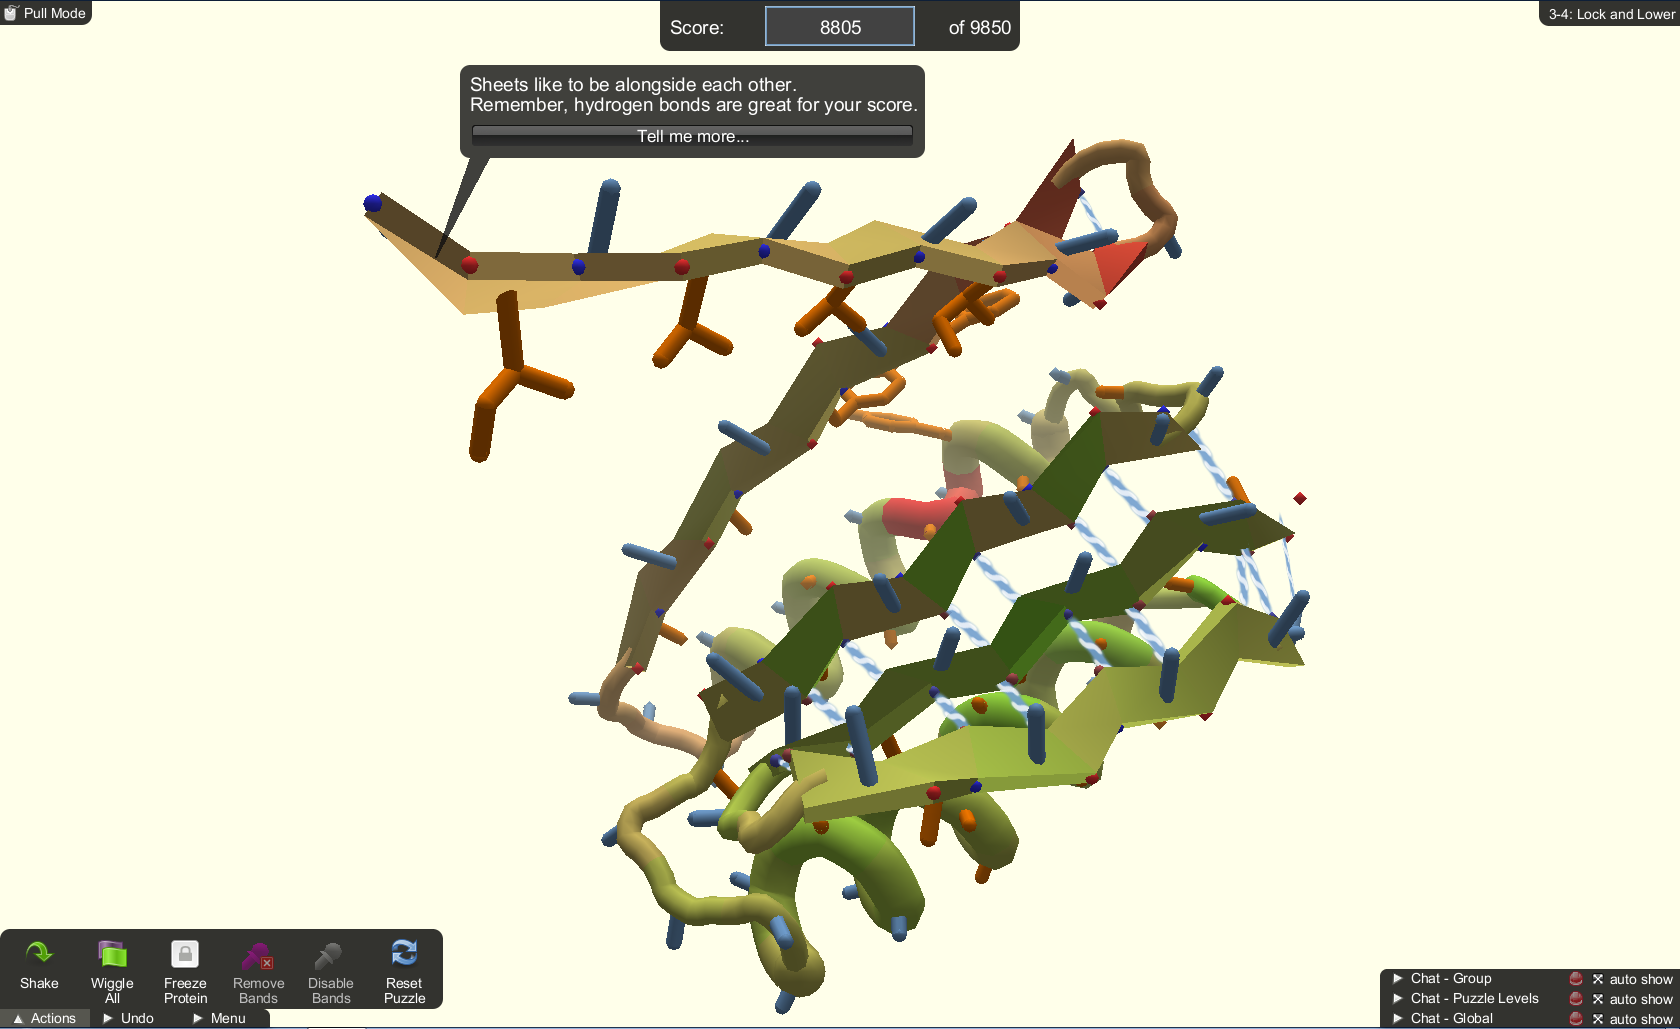
\includegraphics[scale=0.25]{foldit.eps}
		\caption{Foldit is solving a serious problem}
		\label{fig:foldit}
\end{figure}

Serious Alternative Reality Game (ARG) is one type of serious game that blends the real and virtual worlds activities in the serious gaming context.
Jane McGonigal designed the award winning serious ARG games 
``World Without Oil'' \cite{worldwithoutoil} and ``Evoke''
\cite{urgentevoke} with the goal to empower people to come up with creative
solutions to our most urgent real-world problems. ARGs have also been used to
support learning. Connolly et al. discuss the development of an educational ARG
to motivate secondary school students across Europe to learn foreign languages
\cite{connolly2009arguing}. The results of the pilot run of the game in 2009
indicated that 92\% of students felt the game motivated students to learn a
second language. One of problems the team identified is the limitation of
Moodle platform the game is based on.

The report of the ARGOSI project provides insights to the use of ARGs in game
based learning and the challenges in the field of higher education
\cite{whitton2009alternate}. The pilot was run at the University of Bolton with
the aim to provide an engaging alternative to traditional methods of
introducing students to university life. The overall up-take of the game was
fairly low with 173 players and 23 (13\%) of whom were active. The project
identifies a number of questions surrounding educational ARGs, such as
motivation, relationship to curriculum, marketing and timing. The report
suggests that a complete ARG model may not be appropriate for wholesale
learning, but there is certainly potential in using game elements.

\section{Gamification}

``Gamification'', as defined in \cite {Deterding2011mt}, is ``the use of game design elements in non-game contexts''. 
There are many examples of applications that effectively employ game design elements. We will only briefly examine a few here for the purpose of better understanding the gamification concept and how it is utilized across a wide range of everyday life. 

Nike+ \cite{nikeplus} is a social running game-like application that employs game mechanics to encourage runners - both casual and hardcore - to compete and improve their fitness, with the goal to solve the main problem of most fitness programs: motivation. Nike+ makes it easy for runners to upload their exercise data to its web site, and start challenging themselves and their friends. They can also get supports from their friends through the web site. The game makes running and exercise fun.

\begin{figure}[htbp]
	\centering
		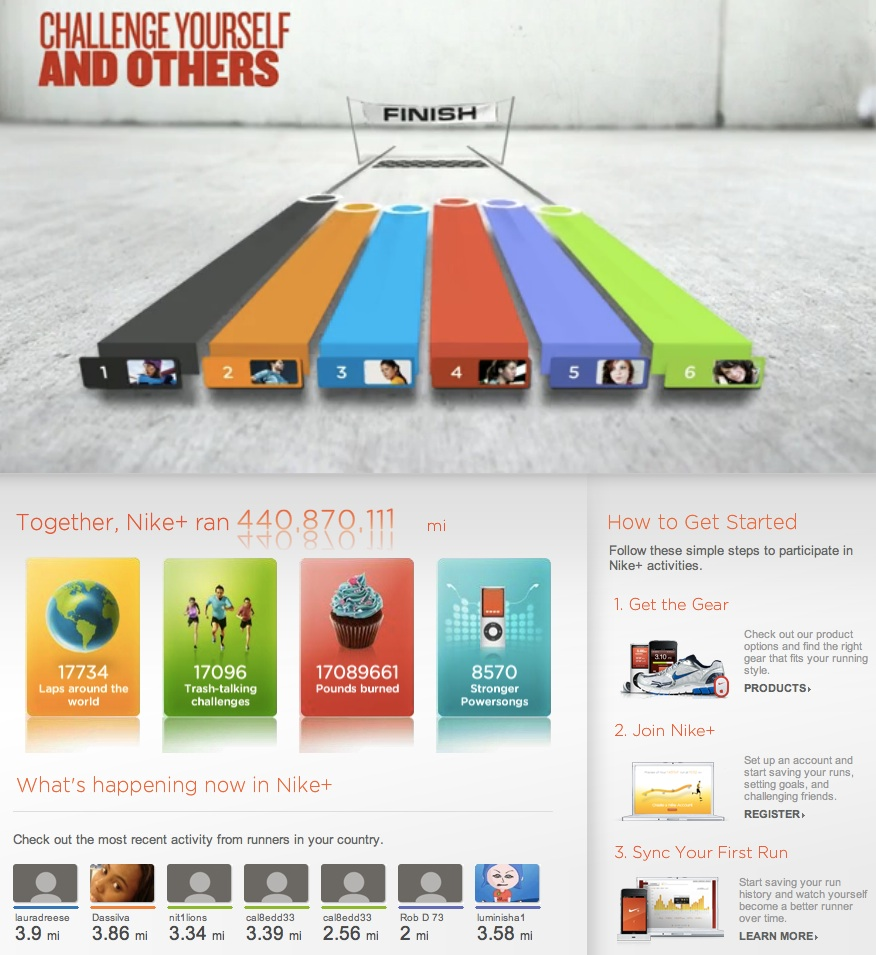
\includegraphics[scale=0.21]{nikeplus.eps}
		\caption{Nike+ makes fitness run}
		\label{fig:nikeplus}
\end{figure}

RibbonHero \cite{ribbonhero} is a game that helps users discover new Microsoft Office features in a fun and motivating way. The goal is to have users build familiarity and expose them to the Office UI, so that they understand what kind of features are available. According to the creator of the game, Office ``has a lot of powerful features that users might not know but can be really useful''. The game gives users a chance to learn those features in a fun and engaging way, rather than reading the software manuals or watching the typically dry IT training videos.

\begin{figure}[htbp]
	\centering
		\subfigure[Quest to earn points]{\label{fig:Ribbon1}\includegraphics[height=2in]{ribbon1.eps}}
		\subfigure[Competing a task]{\label{fig:Ribbon2}\includegraphics[height=2in]{ribbon2.eps}}
		\caption{RibbonHero Helps to Learn Office}
		\label{fig:ribbon}
\end{figure}

The "SmartGauge" dashboard for Ford's hybrid cars, where a digital plant is responding to how energy-efficient the users driving behavior is \cite {ideo2009}. The design gives drivers a game like interaction that for them, the game to grow more lush and beautiful leaves, a visual reward, by driving efficiently, desired behavior. 

Another example is the "Piano Staircase" created by Volkswagen Sweden and ad agency DDB, installed in a metro station in Stockholm \cite {funtheory2009}. The design is to make the staircase next to the escalator look and respond like a piano keyboard, so that every step on the stair will generate different piano sounds every time a commuter walked on it. Observation indicates that 66 percent more people chose the staircase over the escalator, a good example of a "Fun Theory" design for persuading and encouraging energy-efficient behavior.

 \begin{figure}[htbp]
	\centering
		\subfigure[Efficiency Leaves]{\label{ixd-dashbard}\includegraphics[scale=0.3]{ixd-dashboard.eps}}
		\subfigure[Piano Stair vs. Escalator]{\label{fig:ixd-pianostair}\includegraphics[scale=0.35]{ixd-pianostair.eps}}
		\caption{Examples of Gameful Design in Every Day Life}
		\label{fig:ixd}
\end{figure}	

Why game? Results of a study published in the May 1998 issue of Nature \cite {koepp1998evidence} demonstrated that video game players experienced regular releases of dopamine during game play. Dopamine is a
neurotransmitter that signals pleasure rewards for food, sex and addictive drugs, such as cocaine. This and subsequent studies have proven that playing games stimulates pleasure centers in the brain. People are hard-wired to enjoy games.

In the British Museum's department of Greek and Roman antiquities, there is an exhibition section about ancient games. The description of the exhibition states that ``We know very little about how most ancient games were played. Their rules were probably too familiar for people to take the trouble of writing them down''.  A favorite subject of Greek vase-painters was Ajax and Achilles playing a kind of board game called backgammon as illustrated in Figure \ref{fig:ancient-games}. It is noteworthy that both Ajax and Achilles have the full armor on while playing the game. According to Arthur A. Krentz, Plato's ``Republic'' described the connection between play and education of both adult and children. He points out that, the term ``paideia" (in Greek, means education/culture), ``paidia" (means play/game/pastime/sport), and ``paides" (means children), have the same root. The three terms often show up in the same context. ``The central aim of pedagogy (paidagogia) is to encourage learning as a form of play (paidia), which is the most persuasive and effective approach to learning" \cite{krentz1998play}.

\begin{figure}[htbp]
	\centering
		
\includegraphics[scale=0.4]{roman-game-vase.eps}
		\caption{Ancient Games Shown in British Museum}
		\label{fig:ancient-games}
\end{figure}

In modern day, World of Warcraft (WoW) is a massively multiplayer online role-playing game (MMORPG) with 11.1 million subscribers, currently the world's most popular MMORPG.  More than 50 billion hours have been spent in playing the game since the start of this game in 2004. The players created 250,000 articles in the WoW-Wiki, the second largest wiki behind Wikipedia. On average each WoW-player spends from 17 to 21 hours per week playing WoW.

Nick Yee pointed out that the shared experience, the collaborative nature of most activities makes MMORPG unique. ``It's the people that are addictive, not the game''. ``Most importantly, it is the reward of being socialized into a community of gamers and acquiring a reputation within it''  \cite {yee2002understanding}. He claimed that ``WoW truly is a virtual Skinner box'', smoothly increasing reward and difficulty and reinforcing player commitment along the way \cite {yee2001vsb}. 
	
In her popular and inspiring TED talk ``Gaming can make a better world" \cite {mcgonigal2010ted} and in her book ``Reality is Broken" \cite {mcgonigal2011reality}, researcher and game designer Jane McGonigal illustrated why good games make us better, and how they can help us change the world. She notes that currently more than 3 billion hours a week is spent in playing video game by our society, for good reasons. She says that the average gamer plays 10,000 hours of games by age 21. That?s about the same number of hours that students spent in high school and middle school. There are 500 million gamers today, playing on all sorts of platforms from the iPhone to the game consoles. Instead of the common conception that gaming is a waste of time, she argues that ``playing games is the single most productive thing we can do with our time'' and is the solution to the ``Broken Reality". 

In order to understand why people play games, Richard Bartle identified four player personality types by studying players of the Multi-User Dungeon (MUD) game in 1960s \cite {bartle1996hearts}. The four types are based on the 2 underlying axes:

1. Achievers: driven by in-game goals, usually some form of points gathering - whether experience points, levels, or money.

2. Explorers:  driven to find out as much as they can about the virtual construct - including mapping its geography and understanding the game mechanics.

3. Socializers: use the virtual construct to converse and role-play with their fellow gamers.

4. Killers: use the virtual construct to cause distress on other players, and gain satisfaction from inflicting anxiety and pain on others.

Bartle's player type model has been the basic for understanding the player motivation. Dan Dixon presented the limitation and misuse of Bartle's model in general games and gamification contexts \cite{DixonPlayerType}. Amy Jo Kim applied the model in her gamification approach by overlaying social actions from the game on top of the player types \cite {Kim2010}, as shown in Figure 2.8.

\begin{figure}[htbp]
	\centering
		\subfigure[Bartle's Player Types (1996)]{\label{fig:player-types}\includegraphics[height=2.0in]{bartle-player-types.eps}}
		\subfigure[Kim's Social Actions (2010)]{\label{fig:social-action}\includegraphics[height=2.0in]{kim-player-types.eps}}
		\caption{Player Types}
		\label{fig:play-types}
\end{figure}

There are many debates and criticism over whether gamification itself is inherently good or bad. 
Many considered the current efforts of gamification focus on extrinsic motivators (such as points, badges and rewards) instead of intrinsic motivators generated by an individual's internal will or desires.

Designer Stephen Anderson claimed that \cite {anderson2011} gamification mistakes extrinsic rewards (rather than intrinsic motivation) for the power of games and hence offers only feedback, not goals \& rules. 

\begin{figure}[htbp]
	\centering
		\includegraphics[scale=0.25]{anti-gamification.eps}
		\caption{Gamification is about extrinsic rewards (source: Anderson \cite {anderson2011})}
		\label{fig:anti-gamification}
\end{figure}

Jane McGonigal spoke about her concern about current state of gamification in the GDC 2011 talk titled ``We don't need no stinking badges: How to reinvent reality without gamification'' \cite {mcgonigal2011}. She argued that current gamification confuses intrinsic/extrinsic motivation and proposed ``Gameful Design'' instead of ``Gamification''. She claimed that "Gameful is player-oriented", which presumed that the loyalty program type gamification is product or service oriented. While the current gamification is about extrinsic reward, with points, badges, and levels, gameful design is about intrinsic reward, with positive emotion, relationships, meaning and accomplishment.

Nicole Lazzaro argued that the use of extrinsic rewards will decrease the motivation to use your products and services once you remove that reward \cite {Lazzaro2011}. Vockell resonated that in education psychology, extrinsic motivators may lead to short-range activity increase but reduction in long-range interest in a topic. While intrinsic motivators motivate people best when they are working toward personally meaningful goals \cite{vockell2004educational}. 

Michael Wu argues that extrinsic rewards can jumpstart intrinsic motivation  \cite {WuSustainable2011}. He claimed that gamification just has to work long enough for some other processes to take over as the primary driver of value. Subsequently, it becomes a secondary reinforcement system. 

As we discussed before, gamification's main driving force is motivation. Serious games also try to solve the motivation problem and influence people's behavior.  Deterding illustrates the distinctions between gamification, serious games and other related concepts, As shown in Figure 2.15 \cite {Deterding2011mt}.

\begin{figure}[htbp]
	\centering
		\includegraphics[scale=0.55]{defining_gamification.eps}
		\caption{Serious Game and Gamification (source: Deterding \cite{Deterding2011mt})}
		\label{fig:define_gamification}
\end{figure}

According to Deterding, a) Gamification is about game. It is different than playful interaction, playful design. b) Gamification uses game elements. It is not the complete game such as a serious game. c) Gamification applies to non-game context. Similar to serious game, it uses game for other purposed than game's normal expected use for entertainment. d) Gamification focuses on design. It is not game-based technology or practice of wider game ecology.

The difference between Gamification and Serious game is not very clear. Both are trying to solve a problem with game thinking. Some reference serious game such as Foldit as a victorious example of gamification in science \cite{bosch2011}. Sebastian Deterding's definition \cite {Deterding2011mt} illustrates that gamification are total different than serious game.

\section{Serious Games for Sustainability}

Energy competitions or challenges have been introduced to college dormitories
and residential homes as ways to facilitate and incentivize energy reduction.
Petersen et al. describe their experiences deploying a real-time feedback
system in an Oberlin College dorm energy competition in 2005 that includes 22
dormitories over a 2-week period \cite{petersen-dorm-energy-reduction}. Web
pages were used to provide feedback to students. They found a 32\% reduction in
electricity use across all dormitories. However, in a post-competition survey,
respondents indicated that some behaviors, such as turning off hallway lights
at night and unplugging vending machines were not sustainable outside the
competition period.  Overall, there has been little analysis on energy usage
after competitions finish, or how positive behavior changes could be sustained.

\begin{figure}[htbp]
	\centering
		
\includegraphics[scale=0.3]{oberlin.eps}
		\caption{Oberlin Energy Competition}
		\label{fig:oberlin}
\end{figure}

Reeves et al. described the design of Power House, an energy game that connects
home smart meters to an online multiple player game with the goal to improve
home energy behavior \cite{Reeves2011powerhouse}. In the game, the real world
energy data are transformed into a ``more palatable and relevant form of
feedback'', and players may be incentivized by the in-game rewards to complete
more energy-friendly real-world behaviors.

\begin{figure}[htbp]
	\centering
		\includegraphics[scale=0.3]{powerhouse.eps}
		\caption{Power House (source: Reeves \cite{Reeves2011powerhouse})}
		\label{fig:powerhouse}
\end{figure}

RecycleBank \cite {recyclebank} introduced a series of ``Green Challenges'' that used gaming techniques online to motivate participants to learn about green living and to take small green actions to live more sustainable lives offline. According to their report \cite {gamingforgood}, 49,000 individuals participated in the ``Green Your Home Challenges''. Partnered with Google Analytics and ROI research, they found that:
\begin{itemize}
	\item Gamification can increase awareness of positive environmental actions. 97\% of participants surveyed said the game increase their knowledge of environment.
	\item Games can drive individuals to take positive social and environmental actions. Most participants surveyed indicated they are very or extremely likely to take green actions as a result of participating in the challenge.
	\item Games are an effective and appealing educational tool. 86\% participants agreed online games and contest can be a good way to inform and educate them personally.
\end{itemize}

\begin{figure}[htbp]
	\centering
		\subfigure[Green Your Home Challenge]{\label{fig:RecycleBank1}\includegraphics[scale=0.3]{recyclebank1.eps}}
		\subfigure[Game Change Behavior]{\label{fig:RecylceBank2}
\includegraphics[scale=0.65]{recyclebank2.eps}}
		\caption{RecycleBank - Gaming for Good}
		\label{fig:recyclebank}
\end{figure}

\section{Serious Game Frameworks}

Game frameworks (also known as game engines) are ``comprised of a collection
of different tools, utilities, and interfaces that hide the low-level details of the
various tasks that make up a game''~\cite{sherrod2006ultimate}. One of the benefits of
using a serious game framework is that, if correctly designed, it will provide useful and
reusable ``building blocks'' with which to develop a variety of serious games.  These
building blocks enable the serious game developer to focus more time and thought on
content and results instead of on infrastructure.

The examples of game engine includes:
\begin {itemize}
    \item FPS: Unreal (rendering, physics, AI)
    \item Mobile: Papaya
    \item Healthcare: OpenLabyrinth
    \item Educational storytelling: Fabula
\end {itemize}

The Building Dashboard \cite{building-dashboard}, developed by Lucid Design
Group, is used to support Oberlin's dorm energy competition,
as well as the Campus Conservation Nationals, a nationwide electricity and
water use reduction competition on college campuses \cite{competetoreduce}.
The Building Dashboard enables viewing, comparing and sharing building energy
and water use information on the web in compelling visual interface, but the
cost of the system creates the barrier for wider adoptions. In addition, the
building dashboard solutions focus on providing energy information as
a passive media. Besides a scoreboard, There is little interaction between participants
and the system.

\begin{figure}[htbp]
	\centering
		
\includegraphics[scale=0.6]{building-dashboard.eps}
		\caption{Building Dashboard (source: Lucid \cite{building-dashboard})}
		\label{fig:building-dashboard}
\end{figure}

The Stanford Energy Services Platform \cite{Armel-2012} provides services to benefit the creations of energy efficiency program and research. The services include data storage, recommendation system,
user registration and participation assignment, surveys and analytics. It had been utilized to support
the implementation of several Stanford's energy saving projects. such as Power House, Power Down,
Energy Calculator.

\begin{figure}[htbp]
	\centering
		
\includegraphics[scale=0.4]{stanford-esp.eps}
		\caption{Stanford Energy Services Platform (source: Stanford \cite{Armel-2012})}
		\label{fig:building-dashboard}
\end{figure}

\section{Serious Game Framework Assessment}

One fundamental question in evaluating a serious game is the extent to which the
game achieves its ``serious'' purpose.  This is quite different from 
traditional entertainment games, in which evaluation focuses on usability or
playability~\cite{song2007new}. In the field of serious games, there is an increasing
focus on the methodology of game evaluation~\cite{Mayer2012233}. De Freitas and
Oliver describe a four dimensional framework~\cite{de2006can} for evaluating an
educational game, consisting of: the context, the pedagogy, the representation, and the
learner (or player). Harteveld proposes an alternative approach called ``Triadic Game
Evaluation''~\cite{harteveld2010triadic}, consisting of three perspectives: Reality,
Meaning, and Play.

The above approaches focus on evaluation of a single game, as opposed to a game {\em
  framework}. Game frameworks (also known as game engines) are ``comprised of a collection
of different tools, utilities, and interfaces that hide the low-level details of the
various tasks that make up a game''~\cite{sherrod2006ultimate}. One of the benefits of
using a serious game framework is that, if correctly designed, it will provide useful and
reusable ``building blocks'' with which to develop a variety of serious games.  These
building blocks enable the serious game developer to focus more time and thought on
content and results instead of on infrastructure. Yet how are we to know if a serious
game framework has been ``correctly designed''?

There exists some assessment tools such as GEQ (Game Engagement Questionnaire)\cite{brockmyer2009development}, QUIS (Questionnaire for User Interaction Satisfaction)\cite{harper1993improving}. We found no prior work concerning comprehensive assessment for 
the particular needs of a serious game framework. 